
\documentclass[a4paper,10pt,fleqn, twocolumn]{IEEEtran}
\usepackage{amsfonts}
\usepackage{amsthm}
\usepackage{amsmath}
\usepackage{graphicx}
\usepackage{fancyhdr}


\newtheorem{Prop}{Proposition}
\newtheorem{lemma}{Lemma}
\newtheorem{theorem}{Theorem}

\setlength{\parindent}{3em} \setlength{\oddsidemargin}{0in}
\setlength{\textwidth}{6.5in} % sets 1in left and right margins
\setlength{\topmargin}{0.20in} % change to 0.2in for regular latex
%\setlength{\headheight}{0in}
%\setlength{\footheight}{0.5in}
\setlength{\footskip}{0.5in}
\setlength{\textheight}{9.0in} %sets 1in top and bottom margins
\renewcommand{\baselinestretch}{1} %set to 1.5 for double spacing.

\newcommand{\br}{{\mathbf r}}
\newcommand{\bA}{{\mathbf A}}
\newcommand{\ba}{{\bf a}}
\newcommand{\bb}{{\bf b}}
\newcommand{\bc}{{\bf c}}
\newcommand{\bC}{{\bf C}}
\newcommand{\bd}{{\bf d}}
\newcommand{\be}{{\bf e}}
\newcommand{\bE}{{\bf E}}
\newcommand{\bbf}{{\bf f}}
\newcommand{\bF}{{\bf F}}
\newcommand{\bh}{{\bf h}}
\newcommand{\bH}{{\bf H}}
\newcommand{\bg}{{\bf g}}
\newcommand{\bG}{{\bf G}}
\newcommand{\bq}{{\bf q}}
\newcommand{\bs}{{\bf s}}
\newcommand{\bm}{{\bf m}}
\newcommand{\bn}{{\bf n}}
\newcommand{\bu}{{\bf u}}
\newcommand{\bv}{{\bf v}}
\newcommand{\bw}{{\bf w}}
\newcommand{\bx}{{\bf x}}
\newcommand{\by}{{\bf y}}
\newcommand{\bz}{{\bf z}}
\newcommand{\bL}{{\bf L}}
\newcommand{\bM}{{\bf M}}
\newcommand{\bN}{{\bf N}}
\newcommand{\bS}{{\bf S}}
\newcommand{\bT}{{\bf T}}
\newcommand{\bD}{{\bf D}}
\newcommand{\bX}{{\bf X}}
\newcommand{\bP}{{\bf P}}
\newcommand{\bQ}{{\bf Q}}
\newcommand{\bI}{{\bf I}}
\newcommand{\bR}{{\bf R}}
\newcommand{\bU}{{\bf U}}
\newcommand{\bV}{{\bf V}}
\newcommand{\bW}{{\bf W}}
\newcommand{\bY}{{\bf Y}}
\newcommand{\bZ}{{\bf Z}}
\newcommand{\bJ}{{\bf J}}
\newcommand{\bB}{{\bf B}}
\newcommand{\bzero}{{\bf 0}}
\newcommand{\bgamma}{{\mbox {\boldmath $\gamma$}}}
\newcommand{\btheta}{{\mbox {\boldmath $\theta$}}}
\newcommand{\bvartheta}{{\mbox {\boldmath $\vartheta$}}}
\newcommand{\bDelta}{{\mbox {\boldmath $\Delta$}}}
\newcommand{\bLambda}{{\mbox {\boldmath $\Lambda$}}}
\newcommand{\bPsi}{{\mbox {\boldmath $\Psi$}}}
\newcommand{\bPhi}{{\mbox {\boldmath $\Phi$}}}
\newcommand{\bcA}{{\mbox {\boldmath ${\cal A}$}}}
\newcommand{\bcB}{{\mbox {\boldmath ${\cal B}$}}}
\newcommand{\bcC}{{\mbox {\boldmath ${\cal C}$}}}
\newcommand{\bcD}{{\mbox {\boldmath ${\cal D}$}}}
\newcommand{\bcF}{{\mbox {\boldmath ${\cal F}$}}}
\newcommand{\bcG}{{\mbox {\boldmath ${\cal G}$}}}
\newcommand{\bcL}{{\mbox {\boldmath ${\cal L}$}}}
\newcommand{\bcN}{{\mbox {\boldmath ${\cal N}$}}}
\newcommand{\bcR}{{\mbox {\boldmath ${\cal R}$}}}
\newcommand{\bcS}{{\mbox {\boldmath ${\cal S}$}}}
\newcommand{\bcH}{{\mbox {\boldmath ${\cal H}$}}}
\newcommand{\bcI}{{\mbox {\boldmath ${\cal I}$}}}
\newcommand{\bcO}{{\mbox {\boldmath ${\cal O}$}}}
\newcommand{\bcP}{{\mbox {\boldmath ${\cal P}$}}}
\newcommand{\bcQ}{{\mbox {\boldmath ${\cal Q}$}}}
\newcommand{\bcV}{{\mbox {\boldmath ${\cal V}$}}}
\newcommand{\bcW}{{\mbox {\boldmath ${\cal W}$}}}


\title{MIMO Relay with Finite-Rate Feedback}
\author{LGE Mobile Research\\San Diego, CA 92131}
\date{}
\begin{document}
\maketitle
\begin{abstract}\small
In this paper, the effects of finite-rate CQI feedback on multiple
antenna relay systems are discussed. We start from multi-antenna
beamforming transmission using uniform random codebook and
formulate average SNR loss due to channel quantization error and
limited-sized precoding codebook. After this, consider MIMO relay
with multiple relay nodes and discussion how the relay channel
capacity suffers from this finite-rate feedback and as well as
codebook design.
\end{abstract}

\section{Introduction}
Multiple antenna systems have received much attention for the past
decade or so, due to their promise of higher spectrum efficiency
without increasing transmit power. It is well-known that the
performance and complexity of multiple-input multiple-output
systems can be improved by making the channel state information
(CSI) available at the transmitter. This is achieved through a
special reverselink CSI feedback channel from the receiver. For
example, there are HS-DPCCH and R-CQI channels for 3GPP HSDPA Rel.
6 and 3GPP2 UMB, respectively. However, the CSI received by the
transmitter is not perfect and suffers from various impairments,
including round-trip delay, signal processing errors, transmission
loss, etc.


\section{System Model And Problem Description}

Consider a three-terminal one-hop MIMO relay channel as shown in
Figure~\ref{MIMO_Relay}, where a relay is used to assist the
transmission from source to destination. All terminals in the
relay model are equipped with multiple antennas. The source
transmits (broadcasts) to the relay and destination in channels 0
and 1, individually noted by $\bH_{0}$ and $\bH_{1}$, and the
relay transmits to the destination in channel 2, noted by
$\bH_{2}$. We assume Channels 1 and 2 are orthogonal to each
other. In practice, the two channels should be further divided in
time, frequency or code domain and interference between Channels 1
and 2 can be modelled as colored additive noise if it is
necessary. For fast data transmission and convenient
implementation, division in frequency or code domain appears more
advantageous than division in time. As long as the channel
coherence time is larger than the reciprocal of the channel
coherence bandwidth, all fading channels may be modelled as if
they were frequency flat, through use of multiple narrow-band
carriers (such as orthogonal frequency division multiplexing).
This is the case for most practical environments. Therefore, we
will assume that the MIMO channel responses between the source and
the relay, the relay and the destination, and the source and the
destination, are represented, respectively, by constant (as
opposed to polynomial) matrices $\bH_{1}$, $\bH_{2}$, and
$\bH_{0}$. The transfer function of a non-regenerative relay is
equivalent to a memoryless weighting matrix $\bW$ that transforms
the (baseband) waveform received at the relay to the (baseband)
waveform transmitted from the relay. Furthermore, we assume that
during the transmission of each packet of data, $\bH_{0}$,
$\bH_{1}$, $\bH_{2}$ and $\bW$ remain constant (as opposed to time
varying). The numbers of antennas equipped at the source,
destination and relay are denoted as $M$, $N$ and $L$,
respectively, and thus we can write $\bH_{0}\in\mathbb{C}^{N\times
M}$, $\bH_{1}\in\mathbb{C}^{L\times M}$,
$\bH_{2}\in\mathbb{C}^{N\times L}$ and $\bW\in\mathbb{C}^{L\times
L}$. We assume that all L antennas at the relay can be used for
both receiving and transmitting.

\begin{figure}
\center{
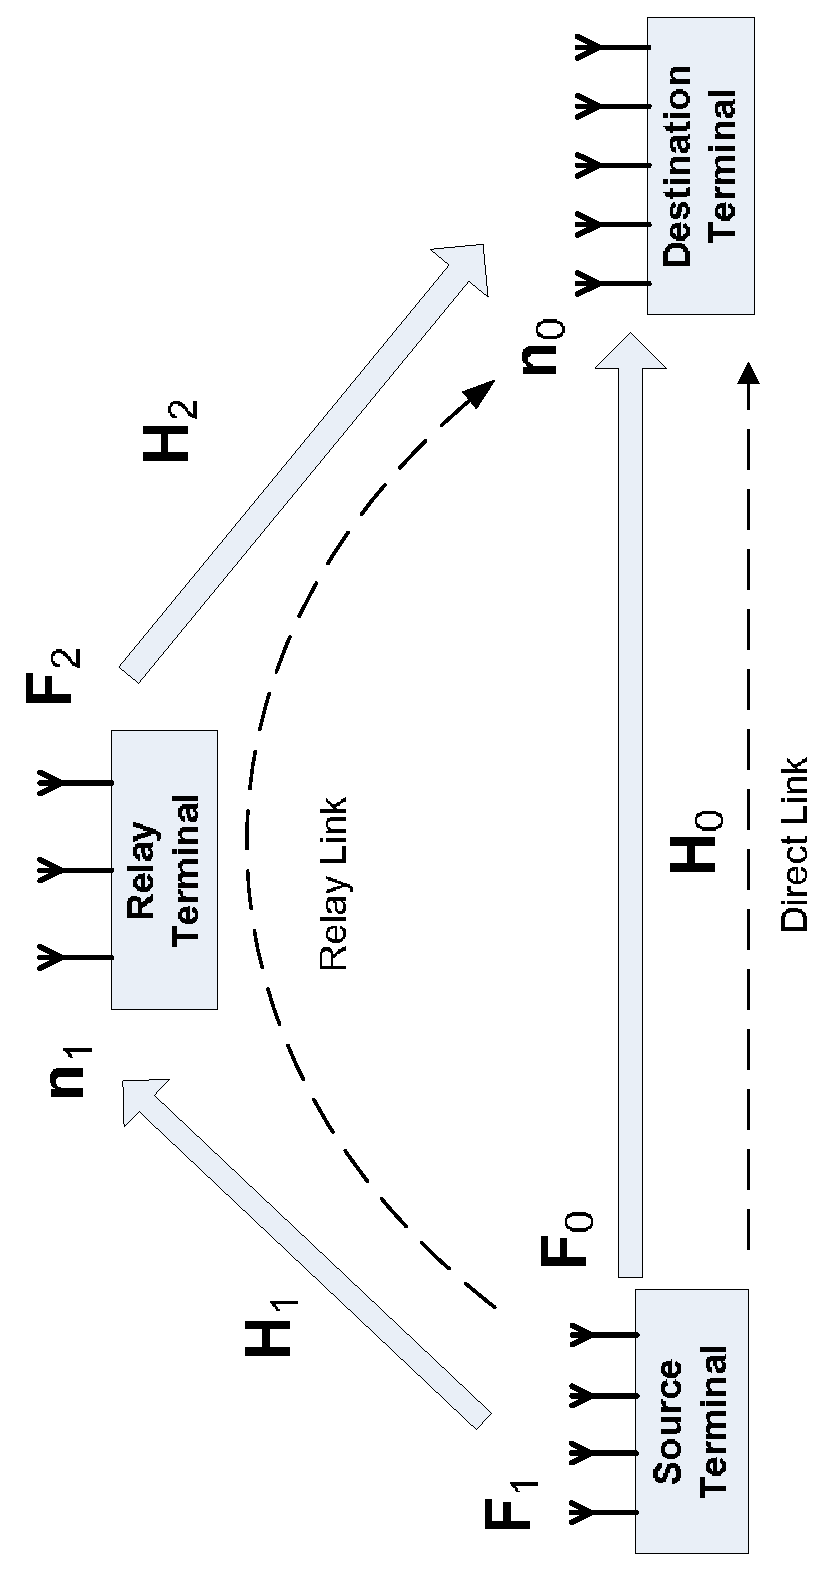
\includegraphics[width=1.5in, angle=270]{MIMO_Relay_01.eps}
\caption{A MIMO relay channel model}\label{MIMO_Relay} }
\end{figure}


If there is no relay link between the source terminal and
destination terminal the MIMO relay channel in
Figure~\ref{MIMO_Relay} becomes a MIMO channel and the received
signals by the destination is
\begin{equation}
\begin{array}{rcl}
\by_{0}& = & \bH_{0}\bW_{0}\bx+\bn_{0}
\end{array}\label{Direct_MIMO}
\end{equation}

\noindent where $\bx$ is the transmitted $M\times 1$ signal vector
by the source with $\bR_{\bx}=\mbox{E}\left\{\bx\bx^{\rm
H}\right\}=\frac{P_{0}}{M}\bI_{M}$, where $\left[\ast\right]^{\rm
H}$ is the Hermitian conjugate operation and $P_{0}$ is the total
transmission power, $\bW_{0}$ is a $M\times M$ MIMO linear
beamforming matrix, and $\bn\sim{\bcC\bcN}(0, \sigma^2\bI_{N})$ is
a complex circular white Gaussian vector. It is well-known that
the achievable MIMO channel capacity is
\begin{equation}
\begin{array}{rcl}
C_{\rm 0}& = &
W\mbox{log}\left|\bI_{N}+\frac{P_{0}}{M}\bH_{0}\bW_{0}\bW_{0}^{\rm
H}\bH_{0}^{\rm H}\right|
\end{array}
\end{equation}
\noindent where $|\ast|$ denotes the determinant of matrix $\ast$.

If we consider the relay link, there are two basic relay modes
among this three-terminal MIMO relay system: 1) Non-Cooperative
MIMO Relay, where the direct link from the source to the
destination and the relay link via the relay terminal are
independent to each other; 2) Cooperative MIMO Relay, where the
direct link and the relay link are cooperatively correlated to
each other. In the following section we give the mathematic models
for these two cases, respectively.

\section{MIMO Relay with Perfect CSI}
If all signals are simultaneously transmitted and relayed using
the same channel resource, the MIMO relay channel can be taken as
a hybrid of a multi-antenna broadcast channel (BC) and a
multi-antenna multi-access channel (MAC). With the assumption that
the relay works in full-duplex mode, dirty paper coding (DPC) and
successive interference cancellation (SIC) are capacity-achieving.
The discussion of the achievable channel capacity for Gaussian
MIMO relay channel and as well as the Rayleigh fading case can be
found in~\cite{WangB05}. In practices, the signals are usually
precoded and transmitted using TDMA, FDMA or CDMA, etc. to
separate the relay link and direct link and possibly the receiving
and transmission at the relay terminal. In the this case, the
signals through the direct link and relay link are orthogonally
separated. The signals received directly through the direct link
is the same as (\ref{Direct_MIMO}) but the relayed signals through
the relay terminal is
\begin{equation}
\begin{array}{rcl}
\by_{1}& = & \bH_{2}\bW_{2}\left(\bH_{1}\bW_{1}\bx+\bn_{1}\right)
+
\bn_{0}\\
& = &\bH_{2}\bW_{2}\bH_{1}\bW_{1}\bx+\tilde{\bn}_{0}
\end{array}
\end{equation}
\noindent where $\bW_{1}$ is the beamforming matrix at the source
terminal and $\bW_{2}$ is the $L\times L$ beamforming matrix at
the relay terminal. $\bn_{1}\sim{\bcC\bcN}(0, \sigma^2\bI_{L})$
denotes the complex circular white Gaussian vector received by the
relay terminal and the $\tilde{\bn}_{0}$ denoted the composite
spatial color noise vector received by the destination terminal
\begin{equation}
\begin{array}{rcl}
\tilde{\bn}_{0} & = & \bH_{2}\bW_{2}\bn_{1} + \bn_{0}
\end{array}
\end{equation}
\noindent with the correlation matrix
\begin{equation}
\begin{array}{rcl}
\bR_{\tilde{\bn}_{0}} & = &
\sigma_{1}^{2}\bH_{2}\bW_{2}\bW_{2}^{\rm H}\bH_{2}^{\rm H} +
\sigma_{0}^2\bI
\end{array}
\end{equation}

The MIMO channel capacity here is
\begin{equation}\hspace{-0.05in}
\begin{array}{rcl}
C&=& \left(1-\alpha\right)C_{0} +  \alpha C_{1}\\
&\hspace{-0.4in}=&\hspace{-0.2in}\left(1-\alpha\right)
W\mbox{log}\left|\bI_{N}+\frac{P_{0}}{M}\bH_{0}\bW_{0}\bW_{0}^{\rm
H}\bH_{0}^{\rm H}\right|+\\
&&\hspace{-0.50in}\alpha
W\mbox{log}\left|\bI_{N}+\frac{P_{0}}{M}\bR_{\tilde{\bn}_{0}}^{+}\bH_{2}\bW_{2}\bH_{1}\bW_{1}\bW_{1}^{\rm
H}\bH_{1}^{\rm H}\bW_{2}^{\rm H}\bH_{2}^{\rm H}\right|
\end{array}\label{MIMO_Relay_Capacity}
\end{equation}
\noindent where $C_{1}$ denote the channel capacity of the relay
link if all resource is allocated for it and it can be written by
\begin{equation}\hspace{-0.0in}
\begin{array}{rcl}
C_{1}&=&\\
&&\hspace{-0.60in}W\mbox{log}\left|\bI_{N}+\frac{P_{0}}{M}\bR_{\tilde{\bn}_{0}}^{+}\bH_{2}\bW_{2}\bH_{1}\bW_{1}\bW_{1}^{\rm
H}\bH_{1}^{\rm H}\bW_{2}^{\rm H}\bH_{2}^{\rm H}\right|\ ,
\end{array}
\end{equation}
\noindent$\alpha\in\left[0\ 1\right]$ denotes the channel resource
partition ratio between the direct link and the total resource in
terms of degree of freedom ( the symbol period multiple the total
bandwidth ) and $\left[\ast\right]^{+}$ denote the pseudo-inverse
of the matrix $\ast$.

In (\ref{MIMO_Relay_Capacity}), the MIMO relay channel capacity is
a balance between direct MIMO and non-regenerative MIMO relay.
When $\alpha=0$, only the direct link exists and the MIMO relay
channel becomes MIMO channel with $C=C_{0}$. When $\alpha=1$, only
the relay link works and the MIMO relay channel becomes
non-regenerative MIMO relay channel with $C=C_{1}$.

\section{MIMO Channel: SINR Degradation with Finite-Rate Feedback}
\begin{figure}
\center{
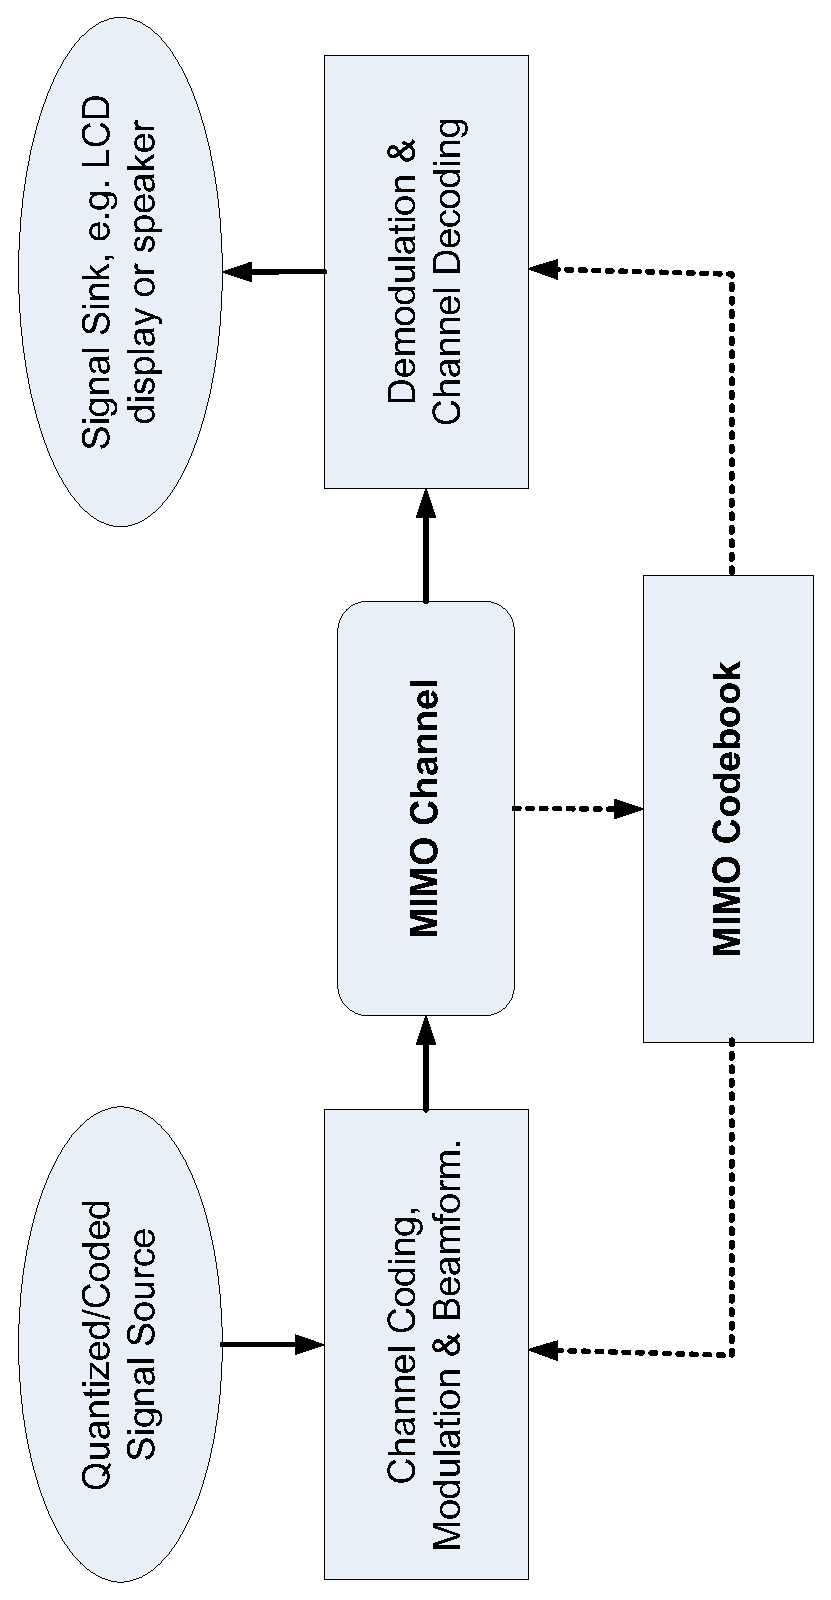
\includegraphics[width=1.5in, angle=270]{MIMO_channel.eps}
\caption{A system model for MIMO with finite-rate
feedback.}\label{MIMO_system} }
\end{figure}

\subsection{Codebook and Channel Quantization}
In a finite-rate feedback model, the receiver estimates channel
responses from each receiving antenna and decides the best
beamforming vector(s) within a MIMO precoding codebook shared
between the receiver and transmitter. This is also called channel
quantization. The receiver then feeds back the chosen precoding
index(es) to the transmitter for the next transmission. The MIMO
beamforming codebook $\bcW$ of the size $2^B$ consists of
$M$-dimensional normalized vectors $\left\{\bw_{1}, ...,
\bw_{2^{B}}\right\}$. It usually takes the receiver $B$ feedback
bits for each beamforming stream. The codebook design usually uses
vector quantization (VQ)~\cite{Narula98} to quantize channel
responses with certain distortion measures. This procedure is also
called Grassmannian line packing~\cite{conway96packing}, which is
similar to spherical packing on unit sphere
$\bcS_{n}\left(1\right)$, where $\bcS_{n}(R)=\left\{\bv:\
\left\|\bv\right\|=R\right\}$ denotes $(n-1)$-sphere. The
Grassmannian space is the space of all $K$-dimensional subspaces
of an $M$-dimensional vector space denoted $\bcG_{k,n}$. The
Grassmannian space $\bcG_{1,n}$ used in Grassmannian line packing
is the space of lines through the origin. Grassmanian can usually
be taken a generalization of projective space.  Obviously
$(n-1)$-unit sphere $\bcS_{n}\left(1\right)$ can be one-to-one
mapped onto $\bcG_{1,n}$. The following conclusion is very
straightforward and it shows that the sphere packing and the
Grassmanian line packing are the same.

\begin{lemma}
For Grassmannian line pack using the metric
\begin{equation}
\begin{array}{rcl}
d_{\rm G}\left(\bv_{1},\ \bv_{2}\right) & = &
\sqrt{1-\left(\bv_{1}^{\rm H}\bv_{2}\right)^{2}}
\end{array},
\end{equation}
\noindent where $ d_{\rm G}\left(\bv_{1},\ \bv_{2}\right)
\in\left[0,\ 1\right]$, is the same to sphere packing using a
squared Euclid distance
\begin{equation}
\begin{array}{rcl}
d_{\rm S}\left(\bv_{1},\ \bv_{2}\right) & = &
\left\|\bv_{1}-\bv_{2}\right\|_2
\end{array},
\end{equation}
\noindent where $d_{\rm S}\left(\bv_{1},\
\bv_{2}\right)\in\left[0,\ \sqrt{2}\right]$.
\end{lemma}

\begin{proof}
If we set the origin of the unit sphere $\bcS_{n}\left(1\right)$
to be the zero point, we may directly take the every point of
$\bcS_{n}\left(1\right)$ as a vector in $\bcG_{1,n}$. And the
relationship between $d_{\rm G}\left(\bv_{1},\ \bv_{2}\right)$ and
$d_{\rm S}\left(\bv_{1},\ \bv_{2}\right)$ is
\begin{equation}
\begin{array}{rcl}
d_{\rm G}^{2}\left(\bv_{1},\ \bv_{2}\right) & = &
1-\left(\bv_{1}^{\rm H}\bv_{2}\right)^{2}\\
&=&1-\left[1-\frac{1}{2}d_{\rm S}^2\left(\bv_{1},\
\bv_{2}\right)\right]^2\ .
\end{array}
\end{equation}
\noindent Obviously the mapping of $d_{\rm G}^{2}\left(\bv_{1},\
\bv_{2}\right)$ to $d_{\rm S}^2\left(\bv_{1},\ \bv_{2}\right)$ is
given by
\begin{equation}
\begin{array}{rcccl}
y&=&f(x)& =&1-\left(1-\frac{1}{2}x\right)^2
\end{array}.
\end{equation}
\noindent Since the differential of $f(x)$ is
\begin{equation}
\begin{array}{rcccl}
\frac{d}{dx}f(x)&=&1-\frac{1}{2}x&>&0
\end{array}
\end{equation}
\noindent for $x\in\left[0,\ 2\right]$, there exists one-to-one
mapping between Grassmannian line packing and sphere packing.
These two spaces are similar to each.

\end{proof}
\subsection{Received SNR Loss}
At the transmitter side, the
signal is precoded by the chosen codeword $\bw_{k}$ following the
feedback from receiver. The received signal then is similar to
(\ref{Direct_MIMO}) but with the distortion $\delta_{i}$ due to
the quantized precoding codeword. This distortion can be expressed
by
\begin{equation}
\begin{array}{rcl}
\delta_{i} & = & \mbox{min}_{\bw\in\bcW}\left\|\bH\bv_{i}-\bH\bw\right\|\\
&=&\lambda_{i}-\mbox{max}_{\bw\in\bcW}\left\|\bH\bw\right\|
\end{array}\label{delta_i}
\end{equation}

\noindent where $\bv_{i}$ denotes the original beamforming vector
for eigen-mode $i$ and $\lambda_{i}$ is the corresponding
eigen-value of $\bH$, which denotes $\bH_{0}$, $\bH_{1}$ or
$\bH_{2}$. It is known that the degradation $\delta_{i}$ is one of
the major sources limiting closed-loop MIMO throughput and the
average SNR distortion decreases with increasing codebook size
$2^B$ . From (\ref{delta_i}), the signal distortion $\delta_{i}$
is a random valuable which depends on $\bv_{i}$, $\bw_{k}$ and
$\lambda_{i}$. The mean of $\delta_{i}$ is
\begin{equation}\hspace{-0.10in}
\begin{array}{rcl}
\bar{\delta}_{i} & = & \mbox{E}\left\{\mbox{min}_{\bw\in\bcW}\left\|\bH\bv_{i}-\bH\bw_k\right\|\right\}\\
& = & \mbox{E}_{\bv_{i}\in{\cal V}_{k}}\left\{\bH\bv_{i}-\bH\bV\bV^{\rm H}\bw_k\right\}\\
&=&\mbox{E}_{\bv_{i}\in{\cal
V}_{k}}\left\{\lambda_{i}\left(1-\bv_{i}^{\rm
H}\bw_k\right)-\sum\limits_{j\neq i}\lambda_{j}\bv_{j}^{\rm
H}\bw_{k}\right\}
\end{array}\label{SNR_degradation}
\end{equation}

\noindent where ${\cal V}_{k}$ denotes the Voronoi cell for
$\bw_{k}$. ${\cal V}_{k}$ is decided by the VQ criteria used in
the codebook design. Different VQ criteria may lead to different
Voronoi decomposition. For example, with Euclid distance criteria,
${\cal V}_{k}$ is defined by

\begin{equation}\hspace{-0.01in}
\begin{array}{rcl}
{\cal V}_{k}&=&\left\{\bv:\|\bv\|=1,\
\frac{\|\bv-\bw_{k}\|}{\|\bv-\bw_{j}\|}<1,\ j\neq k \right\}
\end{array}.\label{Euclid_Voronoi}
\end{equation}

In (\ref{SNR_degradation}) it shows that there are two major
sources causing SNR degradation in MIMO beamforming with imperfect
feedback. The first major source denoted by
\begin{equation}
\begin{array}{rcl}
\Delta_{P}&=&\mbox{E}_{\bv_{i}\in{\cal
V}_{k}}\left|\lambda_{i}\left(1-\bv_{i}^{\rm
H}\bw_k\right)\right|\\
&=&\lambda_{i}\left(1-\mbox{E}_{\bv_{i}\in{\cal
V}_{k}}\left|\bv_{i}^{\rm H}\bw_k\right|\right)\\
&=&\left(1-\alpha_{i}\right)\lambda_{i}\\
\end{array}
\end{equation}

\noindent suggests there is a power degradation and the average
power degradation ratio $\bar{\alpha}_{}$ is
\begin{equation}
\begin{array}{rcl}
\bar{\alpha}_{}&=&\mbox{E}\left\{\alpha_{i}\right\}\\
&=&\mbox{E}\left\{\bv_{i}^{\rm H}\bw_k\right\}\ ,
\end{array}\label{alpha}
\end{equation}

\noindent where $\alpha_{i}=\bv_{i}^{\rm H}\bw_k$.
$\bar{\alpha}_{}$ is irrelevant to the power distribution on the
beams but depends on the codebook design. The second source is the
inter-beam interference (IBI) due to the correlation between the
precoding codeword $\bw_{k}$ and other eigen-modes. It can be
expressed by
\begin{equation}
\begin{array}{rcl}
I_{} & = & \sum\limits_{j\neq i}\lambda_{j}\bv_{j}^{\rm H}\bw_{k}\
\end{array}\label{IBI}
\end{equation}

\noindent  Since we use the uniform random codebook and assume the
MIMO channel response $\bH$ is uniform random too, the eigenvector
$\bv_{j}$ is independent to the eigenvale $\lambda$. The
correlation ratio between $\bw_{k}$ and the $j$th eigen-mode can
be denoted by
\begin{equation}
\begin{array}{rcl}
\alpha_{j}&=&\mbox{E}_{\bv_{i}\in{\cal V}_{k}}\left|\bv_{j}^{\rm
H}\bw_k\right|
\end{array}.\label{alpha_j}
\end{equation}

\begin{Prop}\label{prop_1}
For the uniform random codebook $\bcW$ and isotropically
distributed channel response matrix $\bH$, there is the following
relationship for the correlations defined in (\ref{alpha}) and
(\ref{alpha_j}).

\begin{equation}
\begin{array}{rcccccl}
\alpha + \sum_{j\neq i}\alpha_{j}& = & \alpha + (M-1) \tilde\alpha
& = &1
\end{array},
\end{equation}
\noindent where $\bv_{i}\in{\cal V}_{k}$ and
\begin{equation}
\begin{array}{rcl}
\tilde\alpha&=&\mbox{E}_{j\neq i}\left\{\alpha_{j}\right\}
\end{array}
\end{equation}

\noindent denotes the average interference correlation ratio.

\end{Prop}

With Proposition \ref{prop_1}, the average IBI to other beams in
($\ref{IBI}$) can then be written by
\begin{equation}
\begin{array}{rcccl}
\bar{I}_{}&=& \mbox{E}_{\bv_{i}\in{\cal
V}_{k}}\left\{I\right\}&=&\frac{1-\alpha}{M-1}\sum\limits_{j\neq
i}\lambda_{j}
\end{array}.\label{IBI_2}
\end{equation}

\noindent And the average received SNR $\bar\rho_{i}$ for the
$i$th eigen-mode using codeword $\bw_{k}$ can be written by
\begin{equation}
\begin{array}{rcl}
\bar\rho_{i}&=&\mbox{E}_{\bv_{i}\in{\cal
V}_{k}}\left\{\frac{\lambda_{i}\left(\bv_{i}^{\rm
H}\bw_{k}\right)^2P_{i}}{n_{0}^2+ \lambda_{i}\sum\limits_{l\neq
i}\left(\bv_{i}^{\rm H}\bw_{l}\right)^{2}P_{l}}\right\}\\
&=&\mbox{E}_{\bv_{i}\in{\cal
V}_{k}}\left\{\frac{\lambda_{i}\alpha_{i}^{2}P_{i}}{n_{0}^2+
\lambda_{i}\sum\limits_{l\neq i}\alpha_{l}^{2}P_{l}}\right\}\\
&=&\mbox{E}_{\bv_{i}\in{\cal
V}_{k}}\left\{\frac{\alpha_{i}^{2}\rho_{i}}{1+
\lambda_{i}\sum\limits_{l\neq
i}\frac{\alpha_{l}^{2}}{\lambda_{l}}\rho_{l}}\right\}\ ,
\end{array}
\end{equation}
\noindent where $K\leq\mbox{min}\left\{M,\ N\right\}$ denotes the
number of beams in use and $\rho_{i}$, given by
\begin{equation}
\begin{array}{rcl}
\rho_{i}&=&\frac{\lambda_{i}P_{i}}{\sigma_{0}^2}
\end{array},
\end{equation}

\noindent denotes the maximum achievable SNR




With (\ref{alpha}) the correlation ratio $\alpha$ can be decided
if we know the Voronoi tessellation. However, the closed-form
solution to the boundary of a Voronoi cell, which is a polytope,
generally is unknown, even for a uniform Voronoi tessellation.
This makes it difficult to accurately calculate the average
$\bar{\rho}_{i}$ for the $i$th eigen-mode. Here we suggest an
approach to approximate the Voronoi cell boundary. Instead of
deciding the exact boundary for $\bcV_{i}$, we use a hypercircle
to approximate the bound with the constraint that the interior of
the hypercircle has the same area as the Voronoi cell. In the
following, we details this procedure as well as the theory
principles to decide this hyper-circle. Before doing that, we
present two propositions for calculating the cell area of uniform
Voronoi tessellation and the surface area of hyperspherical cap.

\begin{Prop} The area of a Voronoi cell from a uniform random
codebook of size $2^{B}$ in $M$-dimensional Euclid space is given
by
\begin{equation}
\begin{array}{rcl}
A\left(\bcV_{k}\right)&=&
\frac{2{\pi}^{M}}{2^{B}\Gamma\left(M\right)}
\end{array}\label{V_area}
\end{equation}
\noindent where $\Gamma\left(\ast\right)$ is the gamma function.
\end{Prop}
\begin{proof}
The surface area of a real $n$-ball (the $(n-1)$-sphere) in Euclid
space is
\begin{equation}
\begin{array}{rcccl}
S_{n}\left(R\right)&=&\frac{n}{R}V_{n}&=&\frac{2{\pi}^{\frac{n}{2}}R^{n-1}}{\Gamma\left(\frac{n}{2}\right)}
\end{array}
\end{equation}
\noindent where $V_{n}$ is the volume and $R$ is the radius of the
$n$-ball. A $M$-dimension complex ball in Euclid space with the
radius $R$ is defined by
\begin{equation}\hspace{-0.02in}
\begin{array}{rcccl}
{\bcS}_{M}^{\rm c}\left(R\right)&=&\left\{\bv:\ \left\|\bv\right\|_2=R\right\}&=&\\
&&&&\hspace{-2.20in}\left\{\left[x_{m}+iy_{m}\right]_{M\times1}:\
\sum\limits_{m=1}^{M}(x_{m}^2+y_{m}^2)=R^2\right\}\ .
\end{array}\label{M_complexBall}
\end{equation}

\noindent Therefore, the interior area for the $M$-dimensional
complex ball defined by (\ref{M_complexBall}) is
\begin{equation}
\begin{array}{rcl}
S_{2M}\left(R\right)&=&\frac{2{\pi}^{M}R^{2M-1}}{\Gamma\left(M\right)}
\end{array}.
\end{equation}
\noindent With uniform Voronoi decomposition on ${\bcS}_{M}^{\rm
c}$, we have
\begin{equation}
\begin{array}{rcccl}
S_{2M}\left(1\right)&=&\sum\limits_{k=1}^{2^{B}}A\left(\bcV_{k}\right)&=&2^{B}A\left(\bcV_{k}\right)
\end{array}.
\end{equation}
\end{proof}

After the area of $\bcV_{i}$ is decided by (\ref{V_area}), we
define a $(m-1)$-complex sphere cap $\bcC_{m}^{\rm c}\left(R,\
\psi,\ \bw\right)$,
\begin{equation}\hspace{-0.05in}
\begin{array}{l}
\bcC_{m}^{\rm c}\left(\psi,\ \bw\right)=\left\{\bv:\
\left\|\bv\right\|=\left\|\bw\right\|=R,\ \angle\left(\bv,\
\bw\right)\leq\psi\right\}\ ,\label{M_disk}
\end{array}
\end{equation}
\noindent where $\bw$ is the center of the cap. The solution to
calculate the area of $\bcC_{m}^{\rm c}\left(\theta,\ \bw\right)$
is presented in the following proposition.

\begin{Prop}\label{disk_area} The area of $(m-1)$-complex sphere cap $\bcC_{m}^{\rm c}\left(\psi,\ \bw\right)$ with $\bw=R$ is
\begin{equation}
\begin{array}{rcl}
A\left(\bcC_{m}^{\rm c}\left(\psi,\
\bw\right)\right)&=&\Phi_{m}\left(\psi\right)S_{2m}\left(R\right)
\end{array},
\end{equation}
\noindent where $\Phi_{m}\left(\psi\right)$ is defined by
\begin{equation}
\begin{array}{rcl}
\Phi_{m}\left(\psi\right)&=&1-\cos^{(2m-2)}\left(\psi\right)
\end{array}.
\end{equation}
\noindent And it can be verified that
\begin{equation}
\begin{array}{rcl}
S_{2m}\left(\left\|\bw\right\|\right)&=&A\left(\bcC_{m}^{\rm
c}\left(\pi,\ \bw\right)\right)
\end{array}.
\end{equation}
\end{Prop}

\begin{proof}
At first, a complex hypercircle $\bcO_{m}^{\rm c}\left(r,\
\bc\right)$ on $(m-1)$-complex sphere with radius $R$, the central
point $\bw$ is defined by
\begin{equation}\hspace{-0.00in}
\begin{array}{rcl}
\bcO_{m}^{\rm c}\left(r,\ \bc\right)&=& \bcS_{m}^{\rm c}\left(R\right)\bigcap\bcP_{m}\left(\bc\right)\\
&\hspace{-1.50in}=&\hspace{-0.80in}\left\{\bv:\
\left\|\bv\right\|=R,\ \bc^{\rm H}\left(\bv-\bc\right)=0\
\right\}\ ,
\end{array}
\end{equation}
\noindent where $R=\sqrt{r^2+\|\bc\|_2^2}$. Obviously
$\bcO_{m}^{\rm c}\left(r,\ \bw\right)$ can be taken as a
$(m-2)$-complex sphere and its area is
\begin{equation}\hspace{-0.00in}
\begin{array}{rcl}
A\left(\bcO_{m}^{\rm c}\left(r,\
\bw\right)\right)&=&\frac{2{\pi}^{m-1}r^{2m-2}}{\Gamma\left(m\right)}
\end{array}.
\end{equation}
The area of the complex sphere cap then is
\begin{equation}\hspace{-0.050in}
\begin{array}{rcl}
A\left(\bcC_{m}^{\rm c}\left(\psi,\
\bw\right)\right)&=&\int\limits_{0}^{\psi}A\left(\bcO_{m}^{\rm
c}\left(R\sin\phi,\ \bw\cos\phi\right)\right)d\phi\\
&=&\left[1-\sin^{(2m-2)}\left(\psi\right)\right]S_{2m}\left(R\right)\\
&=&\Phi_{m}\left(\psi\right)S_{2m}\left(R\right)
\end{array}
\end{equation}

\end{proof}

Now the boundary of a Voronoi cell can be approximated by a
hypershpere or a closed space curve decided in the following
lemma.
\begin{lemma}\label{approx_bound} The boundary of the uniform complex Voronoi cell $\bcV_{k}$ can be
approximated by a $(M-1)$-unit complex sphere or a closed complex
space curve.
\begin{equation}\hspace{-0.05in}
\begin{array}{rcl}
\bB\left(\bcV_{k}\right)&\approx& \bcS_{M}^{\rm c}(1)\bigcap \bcL_{M}^{\rm c}(\bw_{k},\ \cos(\theta)) \\
&=&\left\{\bv:\ \left\|\bv\right\|=1,\ \angle\left(\bv,\
\bw_{k}\right)=\theta\right\}\ ,
\end{array}
\end{equation}
\noindent where $\bcL_{M}^{\rm c}\left(\bw_{k},\
\cos(\theta)\right)=\left\{\bv:\ \bv^{\rm
H}\bw_{k}=\cos(\theta)\right\}$ denotes a complex space curve and
$\theta$ is
\begin{equation}\hspace{-0.00in}
\begin{array}{rcl}
\theta&=&\arccos\left(\left(\frac{2^B-1}{2^B}\right)^{\frac{1}{2M-2}}\right)
\end{array}.
\end{equation}

\end{lemma}

From Lemma \ref{approx_bound}, the maximum beamforming power loss
is
\begin{equation}\hspace{-0.00in}
\begin{array}{rcl}
\alpha_{0}&=&\left(\frac{2^B-1}{2^B}\right)^{\frac{1}{2M-2}}
\end{array}.
\end{equation}

\begin{figure}
\center{
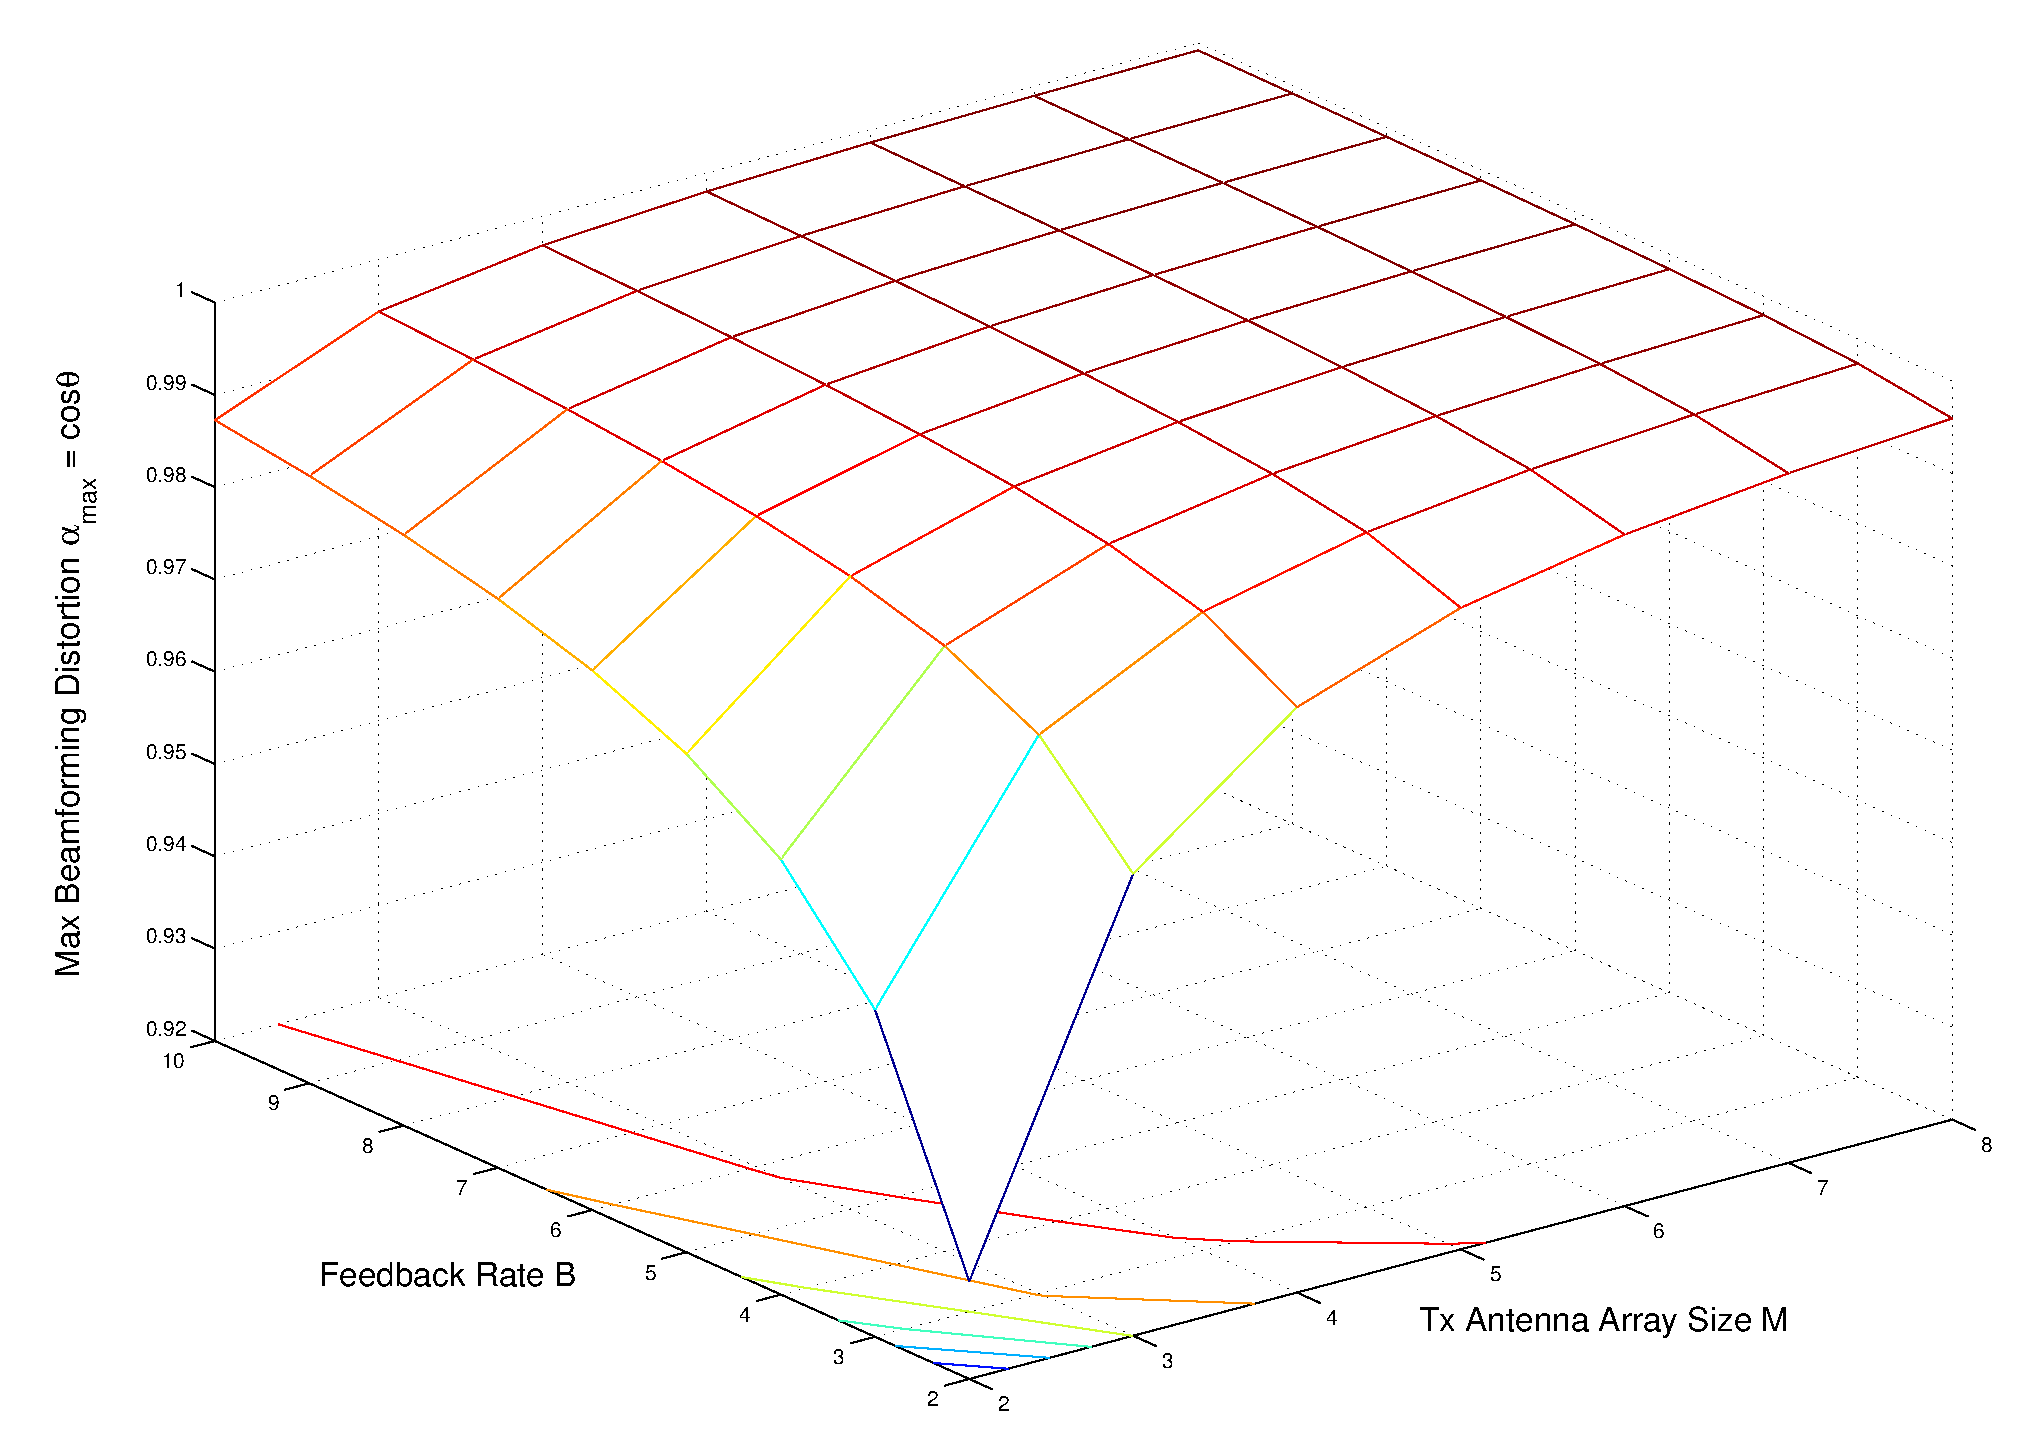
\includegraphics[width=3.20in, angle=0]{MIMO_distortion.eps}
\caption{Approximately maximum beamforming distortion $\alpha$
with various feedback rate $B$ and Tx antenna array size
$M$.}\label{MIMO_distortion} }
\end{figure}


\noindent After the Voronoi boundary is approximately decided, we
need find the probability distribution for beamforming distortion.
In the following lemma, we outline the results for it.

\begin{lemma} The probability density function (PDF) $p\left(\alpha\right)$ and the cumulated density function (CDF) $P\left(\alpha\right)$ of
$\alpha$ are
\begin{equation}\hspace{-0.10in}
\begin{array}{rcl}
p\left(\alpha\right)&=&\mbox{Prob}\left\{x=\alpha\right\}\\
&=&\begin{cases}
0 & 0\leq \alpha < \alpha_{0} \\
\frac{\left(2M-2\right)\alpha\left(1-\alpha^2\right)^{M-2}}{\left(1-\alpha_{0}^{2}\right)^{M-1}}
& \alpha_{0}\leq\alpha\leq 1
\end{cases}
\end{array}
\end{equation}
\noindent and
\begin{equation}\hspace{-0.10in}
\begin{array}{rcl}
P\left(\alpha\right)&=&\mbox{Prob}\left\{x\leq\alpha\right\} \\
&=&
\begin{cases}
0 & 0 \leq\alpha < \alpha_{0} \\
1-\left(\frac{1-\alpha^2}{1-\alpha_{0}^2}\right)^{M-1} &
\alpha_{0}\leq\alpha\leq 1
\end{cases}\ .
\end{array}
\end{equation}
\end{lemma}

\begin{proof}
From Proposition \ref{disk_area}, we have
\begin{equation}\label{Pr_psi}
\begin{array}{rcl}
\mbox{Prob}\left\{\angle(\bv,\
\bw)\leq\psi\right\}&=&\Phi_{M}\left(\psi\right)
\end{array}.
\end{equation}
\noindent Since $\alpha$ is defined by $\alpha =
\cos\left(\angle(\bv,\ \bw\right))$ and
$\alpha\in\left[\alpha_{0},\ 1\right]$, (\ref{Pr_psi}) can be
re-written by
\begin{equation}\label{P_alpha}
\begin{array}{rcl}
\mbox{Prob}\left\{x\geq\alpha\right\}&=&\left(\frac{1-\alpha^2}{1-\alpha_{0}^2}\right)^{M-1}
\end{array}.
\end{equation}
\noindent And we also have
\begin{equation}\hspace{-0.10in}
\begin{array}{rcl}
\mbox{Prob}\left\{x=\alpha\right\}&=&\frac{d}{d\alpha}\mbox{Prob}\left\{x\leq\alpha\right\}\\
&\hspace{-1.80in}=&\hspace{-0.90in}\begin{cases}
0 & 0\leq \alpha < \alpha_{0} \\
\frac{\left(2M-2\right)\alpha\left(1-\alpha^2\right)^{M-2}}{\left(1-\alpha_{0}^{2}\right)^{M-1}}
& \alpha_{0}\leq\alpha\leq 1
\end{cases}
\end{array}.\label{p_alpha}
\end{equation}

\end{proof}

\begin{theorem} The average received SINR for MIMO beamforming with
$B$-bit feedback is
\begin{equation}
\begin{array}{rcl}
\bar\rho_{}&\geq&\frac{\bar{\alpha}^2
P_{0}}{\frac{\sigma_{0}^{2}}{\lambda}+\left(\frac{1-\bar{\alpha}}{M-1}\right)^{2}
\left(P-P_{0}\right)}\ ,
\end{array}
\end{equation}
\noindent where $\lambda$ is the idea channel gain, $K\in\left[1,\
\min\left\{M,\ N\right\}\right]$ denotes the number of selected
beams, $P_0$ is the transmit power for this beam and $P$ is the
total transmit power for all $K$ beams and
\begin{equation}\hspace{-0.05in}\label{alpha_mean}
\begin{array}{rcl}
\bar\alpha&=&\mbox{E}_{\bv_{i}\in{\cal
V}_{k}}\left\{\alpha_{i}\right\}\\
&\approx&\int\limits_{1}^{\alpha_{0}}\frac{\left(2M-2\right)\alpha^2\left(1-\alpha^2\right)^{M-2}}{\left(1-\alpha_{0}^{2}\right)^{M-1}}d\alpha\
.
\end{array}
\end{equation}

\end{theorem}

\begin{proof}

\begin{equation}
\begin{array}{rcl}
\hat{\rho}_{i}&=&\frac{\lambda_{i}\alpha_{i}^{2}P_{i}}{n_{0}^2+
\lambda_{i}\sum\limits_{l\neq i}\alpha_{l}^{2}P_{l}}\\
&\approx&\frac{\alpha_{i}^{2}\rho_{i}}{1+
\frac{1}{M-1}\left(1-\alpha_{i}\right)^{2}\rho_{i}}\\
&=&\Theta\left(\alpha_{i}\right)\ ,
\end{array}
\end{equation}

\noindent where $\Theta\left(x\right)$ is defined by
\begin{equation}
\begin{array}{rcl}
\Theta\left(x\right)&=&\frac{x^{2}\rho_{i}}{1+
\frac{1}{M-1}\left(1-x\right)^{2}\rho_{i}}
\end{array}
\end{equation}
\noindent with $x\in\left[\alpha_{0},\ 1\right]$. It can prove
that $\Theta\left(x\right)$ when $x\in\left[\alpha_{0},\
1\right]$. Following Jensen's inequality, we have

\begin{equation}
\begin{array}{rcl}
\bar{\rho}&=&\mbox{E}\left\{\hat{\rho}_{i}\right\} \\
&=&\mbox{E}\left\{\Theta\left(\alpha_{i}\right)\right\}\\
&\geq&\Theta\left(\bar\alpha_{i}\right)\\
&=& \frac{\bar\alpha_{i}^{2}\rho_{i}}{1+
\frac{1}{M-1}\left(1-\bar\alpha_{i}\right)^{2}\rho_{i}}\ ,
\end{array}
\end{equation}

\end{proof}

It is difficult to give a closed-form solution to $\bar{\alpha}$
in (\ref{alpha_mean}).

\begin{theorem} The bound of the average received SINR satisfy the
following inequality
\begin{equation}\hspace{-0.10in}
\begin{array}{rcccl}
\bar\rho_{i}&\geq& \frac{\sigma_{\alpha}^{2}\rho_{i}}{1+
\frac{1}{M-1}\left(1-\sigma_{\alpha}\right)^{2}\rho_{i}}&\geq&
\frac{\bar\alpha_{i}^{2}\rho_{i}}{1+
\frac{1}{M-1}\left(1-\bar\alpha_{i}\right)^{2}\rho_{i}}\ ,
\end{array}
\end{equation}
\noindent where  $\sigma_{\alpha}$ denotes the standard deviation
of $\alpha$ with $\sigma_{\alpha}^2$ given by

\begin{equation}
\begin{array}{rcl}
\sigma_{\alpha}^2&=&\mbox{E}\left\{\alpha_{i}^2\right\}\\
&=&\int\limits_{1}^{\alpha_{0}}\frac{\left(2M-2\right)\alpha^3\left(1-\alpha^2\right)^{M-2}}{\left(1-\alpha_{0}^{2}\right)^{M-1}}d\alpha\\
&=&\frac{1}{M}+\frac{M-1}{M}\alpha_{0}^2\ .
\end{array}
\end{equation}


\end{theorem}
\begin{figure}
\center{
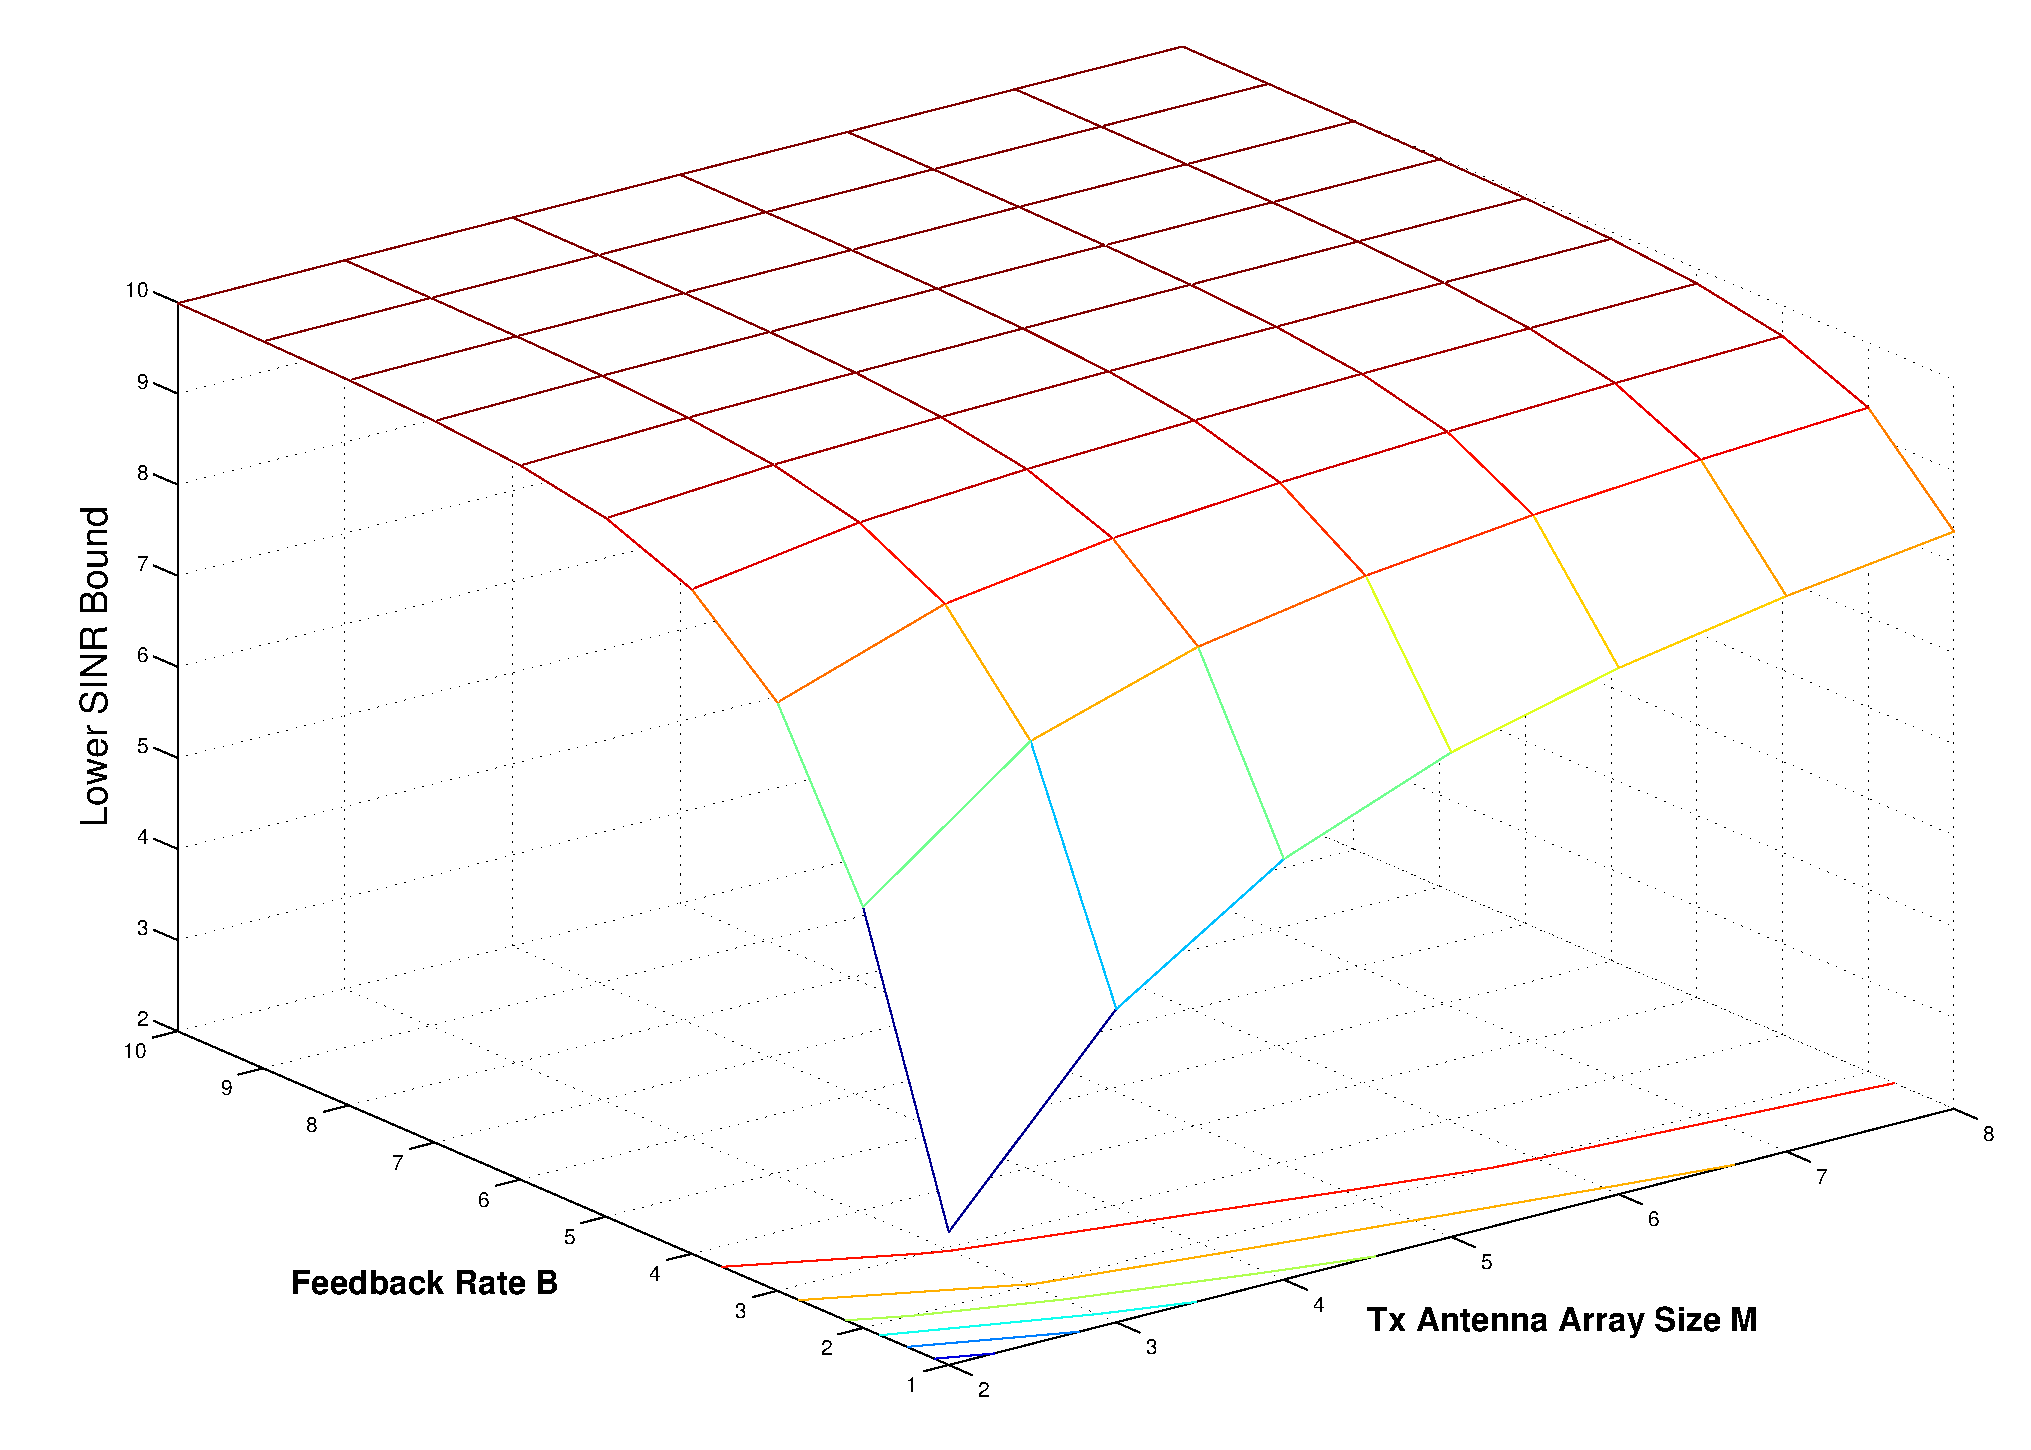
\includegraphics[width=3.20in, angle=0]{MIMO_SNR.eps}
\caption{A lower bound for averaged SINR $\bar\rho_i$ with
$\rho_i=10\text{dB}$ with various feedback rate $B$ and Tx antenna
array size $M$.}\label{MIMO_SINR} }
\end{figure}

\subsection{High-SNR Region}
\begin{theorem} In high-SNR region, MIMO beamforming becomes interference-limited and the average received SINR
is

\begin{equation}\hspace{-0.0in}
\begin{array}{rcl}
 \bar\rho_{i}&\geq&\frac{\bar\alpha_{i}^{2}\rho_{i}}{1+
\frac{1}{M-1}\left(1-\bar\alpha_{i}\right)^{2}\rho_{i}}\\
&\geq&\frac{\left[1-\frac{M-1}{M}\left(1-\alpha_{0}^2\right)\right]^2\rho_{i}}{1+
\frac{M-1}{M^2}\left(1-\alpha_{0}^2\right)^{2}\rho_{i}}\ .
\end{array}
\end{equation}

\end{theorem}

\begin{figure}
\center{
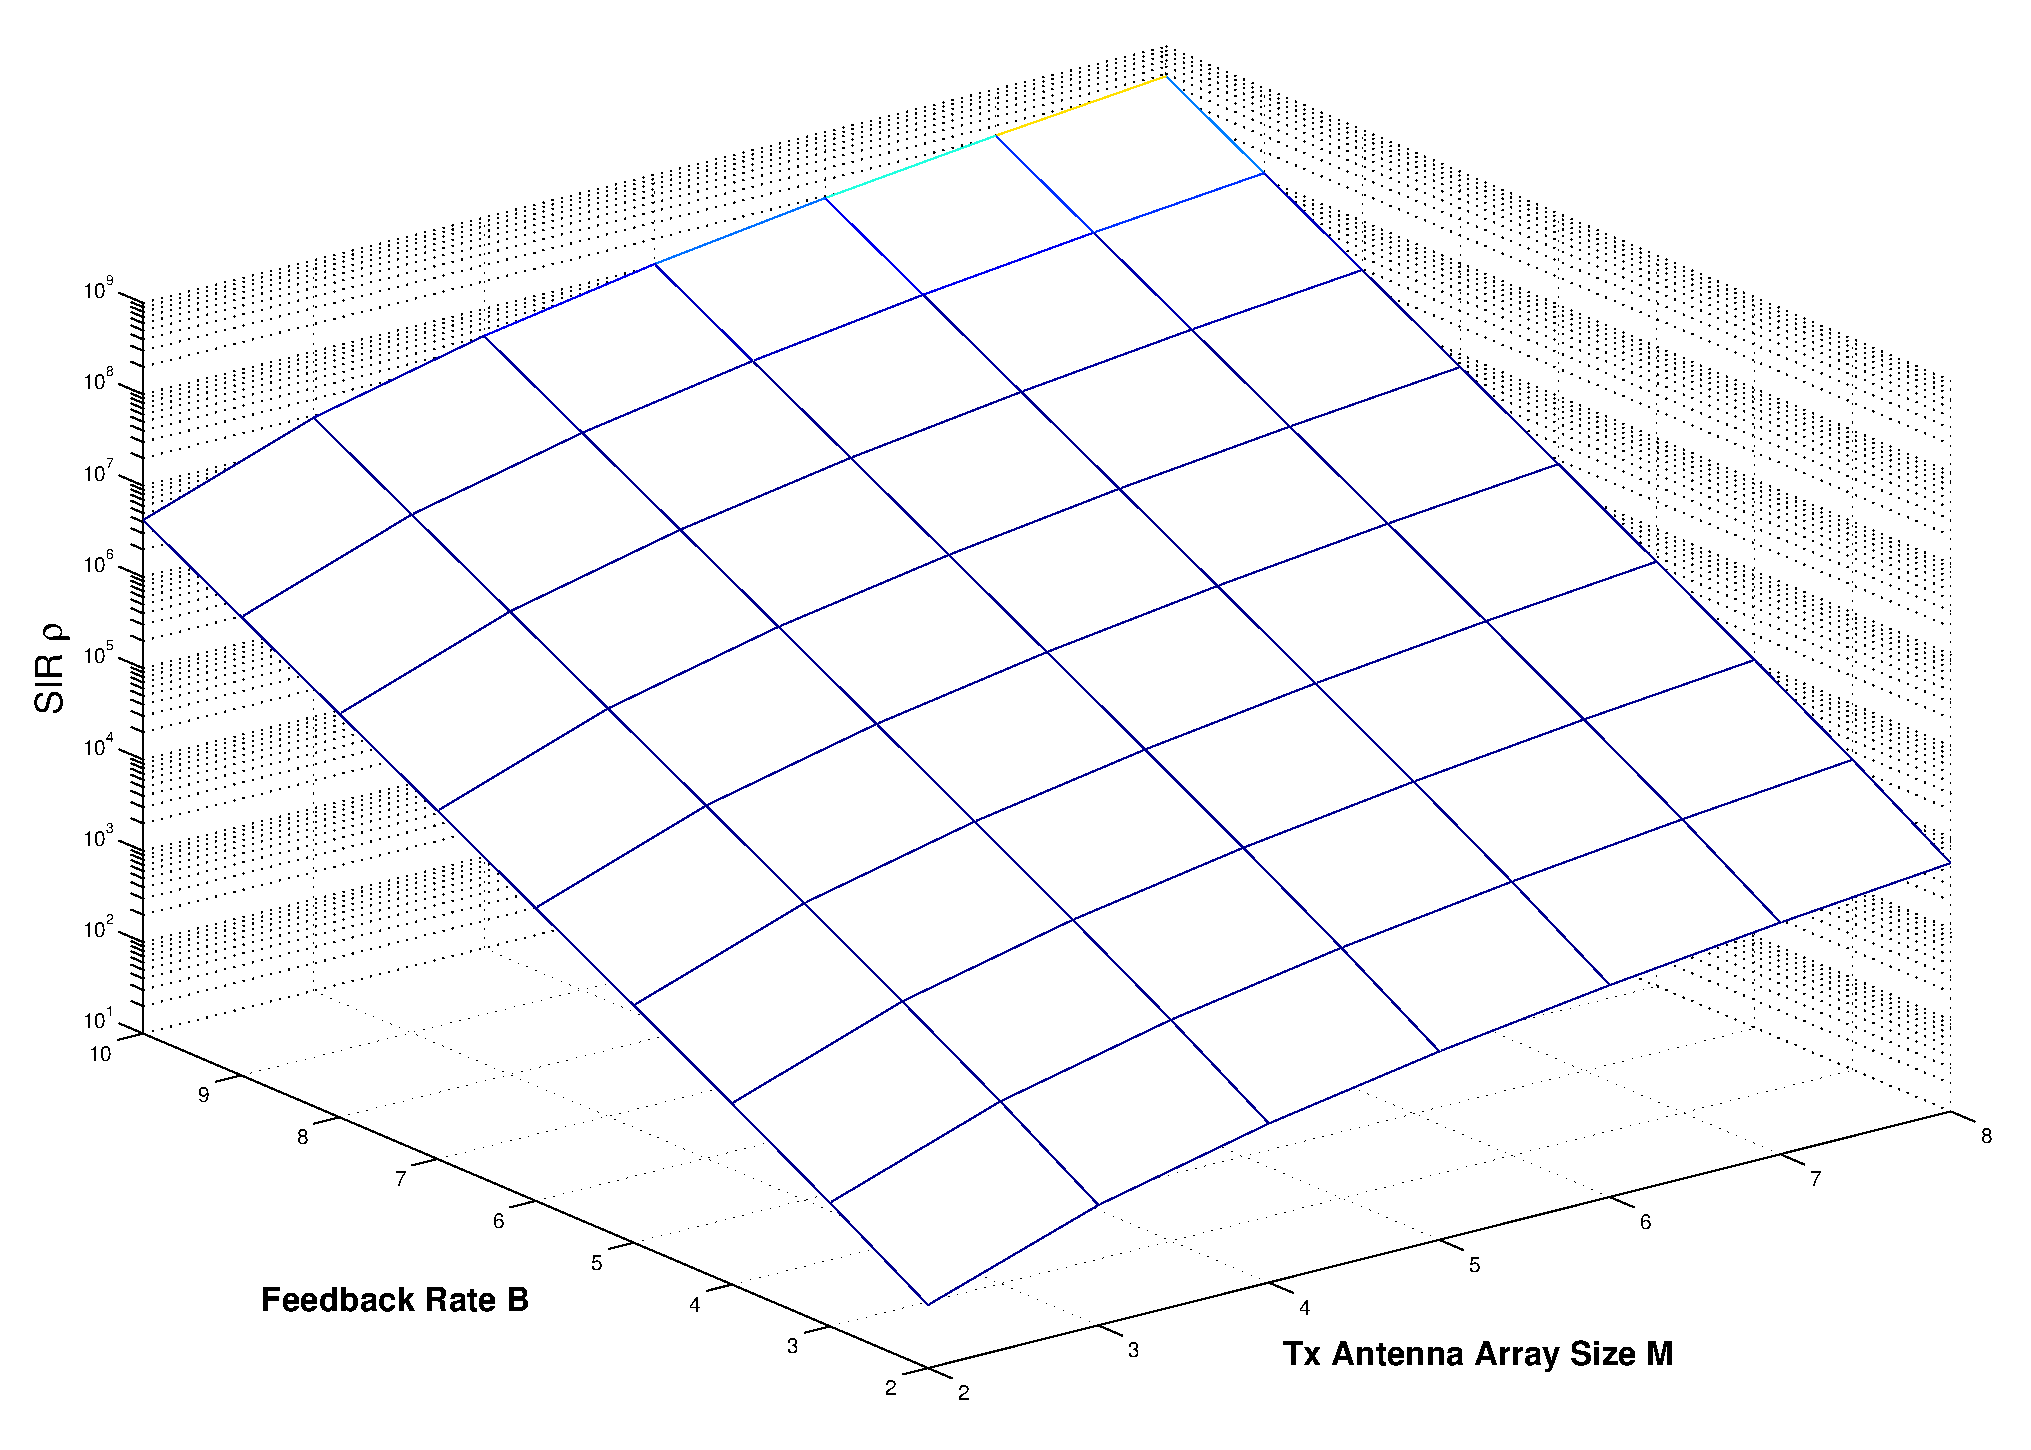
\includegraphics[width=3.20in, angle=0]{MIMO_SIR.eps}
\caption{SIR in high-SNR region with various feedback rate $B$ and
Tx antenna array size $M$.}\label{MIMO_SIR} }
\end{figure}

\section{MIMO Codebook Design for Imperfect Channel Estimation}

\subsection{System Model and Problem Formulation}
Consider $M$-input and $L$-output channels. The channels are
assumed to be frequency-selective block fading, which means the
random channels taps remain constant for some data packets and
change to independent values for the next. The baseband received
signal can be written as:


\begin{equation}\hspace{-0.20in}
\begin{array}{rcl}
\by(t)&=&\left[\begin{matrix}y_{1}(t)\\ y_{2}(t)\\ \vdots \\
y_{L}(t)\end{matrix}\right]\\
&=&\left[\begin{matrix}\sum\limits_{m=1}^{M}h_{m,1}(t)\otimes s_m(t)\\ \sum\limits_{m=1}^{M}h_{m,2}(t)\otimes s_m(t)\\ \vdots \\
\sum\limits_{m=1}^{M}h_{m,L}(t)\otimes
s_m(t)\end{matrix}\right]+\bn\\
&=&\left[\begin{matrix}\bh_{1}^{\rm T}(t)\otimes \bs(t)\\ \bh_{2}^{\rm T}(t)\otimes \bs(t)\\ \vdots \\
\bh_{L}^{\rm T}(t)\otimes \bs(t)\end{matrix}\right]+\bn\ ,
% &=&\bH(t)\otimes\bs(t)+\bn \\
\end{array}
\end{equation}
\noindent where $\bh_{l}(t)=\left[h_{1,l}(t)\ h_{2,l}\ \ldots\
h_{M,l}(t)(t)\right]^{\rm T}$ for $t=0,\ 1,\ \ldots\ L_{c}$ is the
channel impulse response vector from the $m$th transmit antenna to
the $L$ receive antenna and $L_{c}$ is the maximum channel order
for all $L$ subchannels. $s_m(t)$ denotes the transmitted symbol
from the $m$th antenna and $n$ represents the independent additive
Gaussian white noise. Due to the commutativity of convolution, the
stretched discrete received signal vector could as well be
expressed by the following expression

\begin{equation}\hspace{-0.00in}
\begin{array}{rcl}
\by&=&\bS\bh+\bn
\end{array},
\end{equation}

\noindent where $\bh$ is the stretched channel response vector
defined by

\begin{equation}\hspace{-0.00in}
\begin{array}{rcl}
\bh&=&\left[\mbox{vec}(\bH_{1})\ \mbox{vec}(\bH_{2})\ \ldots\
\mbox{vec}(\bH_{M})\right]^{\rm T}
\end{array}
\end{equation}
\noindent with $\bH_{k}=\left[\bh_{k}(0)\ \bh_{k}(1)\ \ldots\
\bh_{k}(L_{c}-1)\right]$ and
\begin{equation}\hspace{-0.00in}
\begin{array}{rcl}
\bS&=&\mbox{kron}\left(\left[\bS_{1}\ \bS_{2}\ \ldots\
\bS_{M}\right]^{\rm T},\ \bI\right)
\end{array}
\end{equation}
\noindent with
\begin{equation}\hspace{-0.10in}
\begin{array}{rcl}
\bS_{k}&=&\left[\begin{matrix}
s_{k}(Q)&\cdots&s_{k}(Q-L_{c})\\
s_{k}(Q-1)&\cdots&s_{k}(Q-L_{c}-1)\\
\vdots&\ddots&\vdots\\
s_{k}(1)&\cdots&s_{k}(1-L_{c})
\end{matrix}\right]
\end{array}.
\end{equation}

Due to pilot design and channel impair,  the

\begin{equation}\hspace{-0.10in}
\begin{array}{rcl}
\bR&=&\bH\bH^{\rm H}
\end{array}.
\end{equation}

When there is an estimation error in $\bR$, the
eigen-decomposition of it becomes

\begin{equation}\hspace{-0.10in}
\begin{array}{rcl}
\hat\bR&=&\sum\limits_{k=1}^{K}\hat{\lambda}_{k}\hat{\bv}_{k}\hat{\bv}_{k}^{\rm
H}
\end{array}.
\end{equation}
The first-order approximation of eigen-values and eigen-vectors is
\begin{equation}\hspace{-0.10in}
\begin{array}{rcl}
\hat\lambda_{k}&=&\lambda_{k}+\hat\bv_{k}^{\rm
H}\bDelta_{\bR}\hat\bv_{k}
\end{array}
\end{equation}
\noindent and
\begin{equation}\hspace{-0.10in}
\begin{array}{l}
\hat\bv_{k}=\bv_{k}+\left(\hat{\bR}-\hat\lambda_{k}\bI\right)^{+}\left[\Delta_{\lambda_{k}}\bI-\bDelta_{\bR}\right]\bv_{k}
\end{array}
\end{equation}
\noindent where
$\Delta_{\lambda_{k}}=\hat{\lambda}_{k}-\lambda_{k}$ and
$\bDelta_{\bR}=\hat\bR-\bR$.


\begin{Prop}
\begin{equation}\hspace{-0.10in}
\begin{array}{rcl}
\left[\bDelta_{\bR}-\Delta_{\lambda_{k}}\bI\right]\bv_{k}&\approx&\sum\limits_{i=1}^{K}\lambda_{i}\bv_{i}\bDelta_{\bv_{i}}^{\rm
H}\bv_{k} + \lambda_{k}\Delta_{\bv_{k}}
\end{array}
\end{equation}
\end{Prop}

\begin{equation}\hspace{-0.30in}
\begin{array}{rcl}
\left(\hat{\bR}-\hat\lambda_{k}\bI\right)\Delta_{\bv_{k}} &\approx
&\sum\limits_{i=1}^{K}\lambda_{i}\bv_{i}\bDelta_{\bv_{i}}^{\rm
H}\bv_{k} + \lambda_{k}\Delta_{\bv_{k}}
\end{array}
\end{equation}

\begin{equation}\hspace{-0.30in}
\begin{array}{rcl}
\alpha_{k}&=&-\hat\bv_{k}^{\rm H}\Delta_{\bv_{k}} \\
&\approx&-\hat\bv_{k}^{\rm
H}\left(\hat{\bR}-\hat\lambda_{k}\bI-\lambda_{k}\bI\right)^{+}\sum\limits_{i=1}^{K}\lambda_{i}\bv_{i}\bDelta_{\bv_{i}}^{\rm
H}\bv_{k}\\
&\approx&\frac{1}{\lambda_{k}}\hat\bv_{k}^{\rm
H}\lambda_{i}\bv_{i}\bDelta_{\bv_{i}}^{\rm H}\bv_{k}

\end{array}
\end{equation}



\subsection{Pilot Design}
\subsubsection{Orthogonal Multiplexed Pilot}

\subsubsection{Superimpose Pilot}



\subsection{Cramer-rao Lower Bound}
The lower bound to the mean-squared errors of unbiased estimates
can be given by the Cramer-Rao bound (CRB), which is defined as
the inverse of the Fisher Information Matrix (FIM). If we denotes
$\bvartheta=\left[\bh^{\rm T}\ \bs_{d}^{\rm T}\right]^{\rm T}$,
the complex FIM is given by

\begin{equation}\hspace{-0.10in}
\begin{array}{rcl}
\mbox{F}\left(\bvartheta\right)&=&\mbox{E}\left\{\left[\frac{\partial\ln\mbox{Pr}\left(\by|\vartheta\right)}{{\partial\vartheta}^{\ast}}\right]\left[\frac{\partial\ln\mbox{Pr}\left(\by|\vartheta\right)}{{\partial\vartheta}^{\ast}}\right]^{\rm H}\right\}\\
 &\hspace{-1.0in}=&\hspace{-0.50in}\sigma_{0}^{-2}\left[\begin{matrix}
\mbox{E}\left\{\bS^{\rm
H}\bS\right\}+\rho_{h}^2\bI&\bzero\\
\bzero&\mbox{E}\left\{\bcH^{\rm H}\bcH\right\}+\rho_{s_{d}}^2\bI
\end{matrix}\right]
\end{array},
\end{equation}
\noindent where
$\rho_{h}^{2}=\mbox{E}\left\{\left|\frac{\partial\ln\mbox{Pr}\left(h\right)}{{\partial
h}^{\ast}}\right|^2\right\}$ and
$\rho_{s_{d}}^{2}=\mbox{E}\left\{\left|\frac{\partial\ln\mbox{Pr}\left(s_{d}\right)}{{\partial
s_{d}}^{\ast}}\right|^2\right\}$.

\subsubsection{Orthogonal Multiplexed Pilot}

\subsubsection{Superimpose Pilot}

\begin{equation}\hspace{-0.10in}
\begin{array}{rcl}
\hat{r}&=&\hat{\bu}^{\rm H}\bH\hat{\bw}s\\
&\hspace{-0.15in}=&\hspace{-0.10in}\left[\bu+\left(\hat{\bu}-\bu\right)\right]^{\rm H}\bH\left\{\bw+\left[Q\left(\hat{\bv}\right)-Q\left(\bv\right)\right]\right\}s\\
&\hspace{-0.15in}\approx&\hspace{-0.10in}\bu^{\rm H}\bH\bw
s+\left({\bf\Delta}_{\bu}^{\rm H}\bH\bw+\bu^{\rm
H}\bH{\bf\Delta}_{\bw}\right)s
\end{array}
\end{equation}



\begin{equation}\hspace{-0.08in}
\begin{array}{rcl}
\bP_{\hat\br}&=&\bH\hat{\bW}\bR_{\bs}\hat{\bW}^{\rm H}\bH^{\rm H}\\
&\hspace{-0.60in}=&\hspace{-0.30in}\bH\left[\bV+\left(\hat{\bW}-\bV\right)\right]\bP_{\bs}\left[\bV+\left(\hat{\bW}-\bV\right)\right]^{\rm H}\bH^{\rm H}\\
&\hspace{-0.60in}=&\hspace{-0.30in}\frac{P}{K}\bH\left[\bV+\left(Q(\hat{\bV})-\bV\right)\right]\left[\bV+\left(Q(\hat{\bV})-\bV\right)\right]^{\rm H}\bH^{\rm H}\\
&\hspace{-0.60in}\approx&\hspace{-0.30in}\frac{P}{K}\bLambda+\frac{P}{K}\bH\left[Q(\hat{\bV})-\bV\right]\bLambda^{\frac{1}{2}}\bU^{\rm
H}\\
&\hspace{-0.00in}&\hspace{-0.00in}+\frac{P}{K}\bU\bLambda^{\frac{1}{2}}\left[Q(\hat{\bV})-\bV\right]^{\rm
H}\bH^{\rm H}
\end{array}
\end{equation}



\begin{equation}\hspace{-0.08in}
\begin{array}{rcl}
\bDelta_{\bv}&=&\hat\bw-\bv \\
&=&Q\left(\hat\bv\right)-\bv \\
&=&\left[Q\left(\hat\bv\right)-\hat\bv\right]+\left(\hat\bv-\bv\right)\\
&=&\left[Q\left(\hat\bv\right)-Q\left(\bv\right)\right]+\left[Q\left(\bv\right)-\bv\right]
\end{array}
\end{equation}


\section{MIMO Beamforming with Interference Cancellation}



\section{MIMO Relay with Finite-Rate Feedback}



\section{Conclusions}

\small
\bibliographystyle{unsrt}
\bibliography{Cooperative_Relay}
\end{document}
